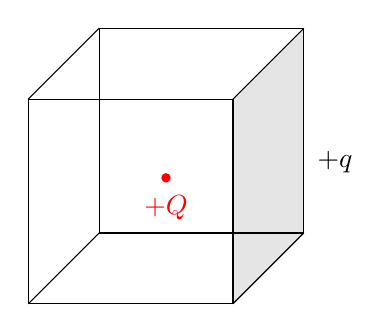
\begin{tikzpicture}
  % cube vertices (front square A B C D, back A2 B2 C2 D2)
  \coordinate (A) at (0,0);
  \coordinate (B) at (2.6,0);
  \coordinate (C) at (2.6,2.6);
  \coordinate (D) at (0,2.6);
  \coordinate (A2) at (0.9,0.9);
  \coordinate (B2) at (3.5,0.9);
  \coordinate (C2) at (3.5,3.5);
  \coordinate (D2) at (0.9,3.5);
  % shaded right face
  \fill[gray!20] (B)--(C)--(C2)--(B2)--cycle;
  % edges
  \draw (A)--(B)--(C)--(D)--cycle;
  \draw (A2)--(B2)--(C2)--(D2)--cycle;
  \draw (A)--(A2); \draw (B)--(B2); \draw (C)--(C2); \draw (D)--(D2);
  % charge inside
  \fill[red] (1.75,1.6) circle (0.06);
  \node[red,below] at (1.75,1.5) {$+Q$};
  % charge on right face
  \node[right] at (3.55,1.8) {$+q$};
\end{tikzpicture}
